\documentclass[../Text/00main.tex]{subfiles}
\graphicspath{{../}}

\begin{document}



\chapter{Additional figures from methods}

\section{Table of CSCS Piz daint specifications}\label{app:pizdaint}

\hl{To do: insert table}

\section{More elaborate workflow description}\label{app:software}

\chapter{Additional result figures}

\section{More images of waveforms from the validation}\label{app:validation}


\section{Additional images of different start configurations}{\label{app:morereffigs}}

\subsection{Reference scenarios CMT3 and CMT4}

\subsubsection{CMT3}

\begin{figure}[h]
    \centering
    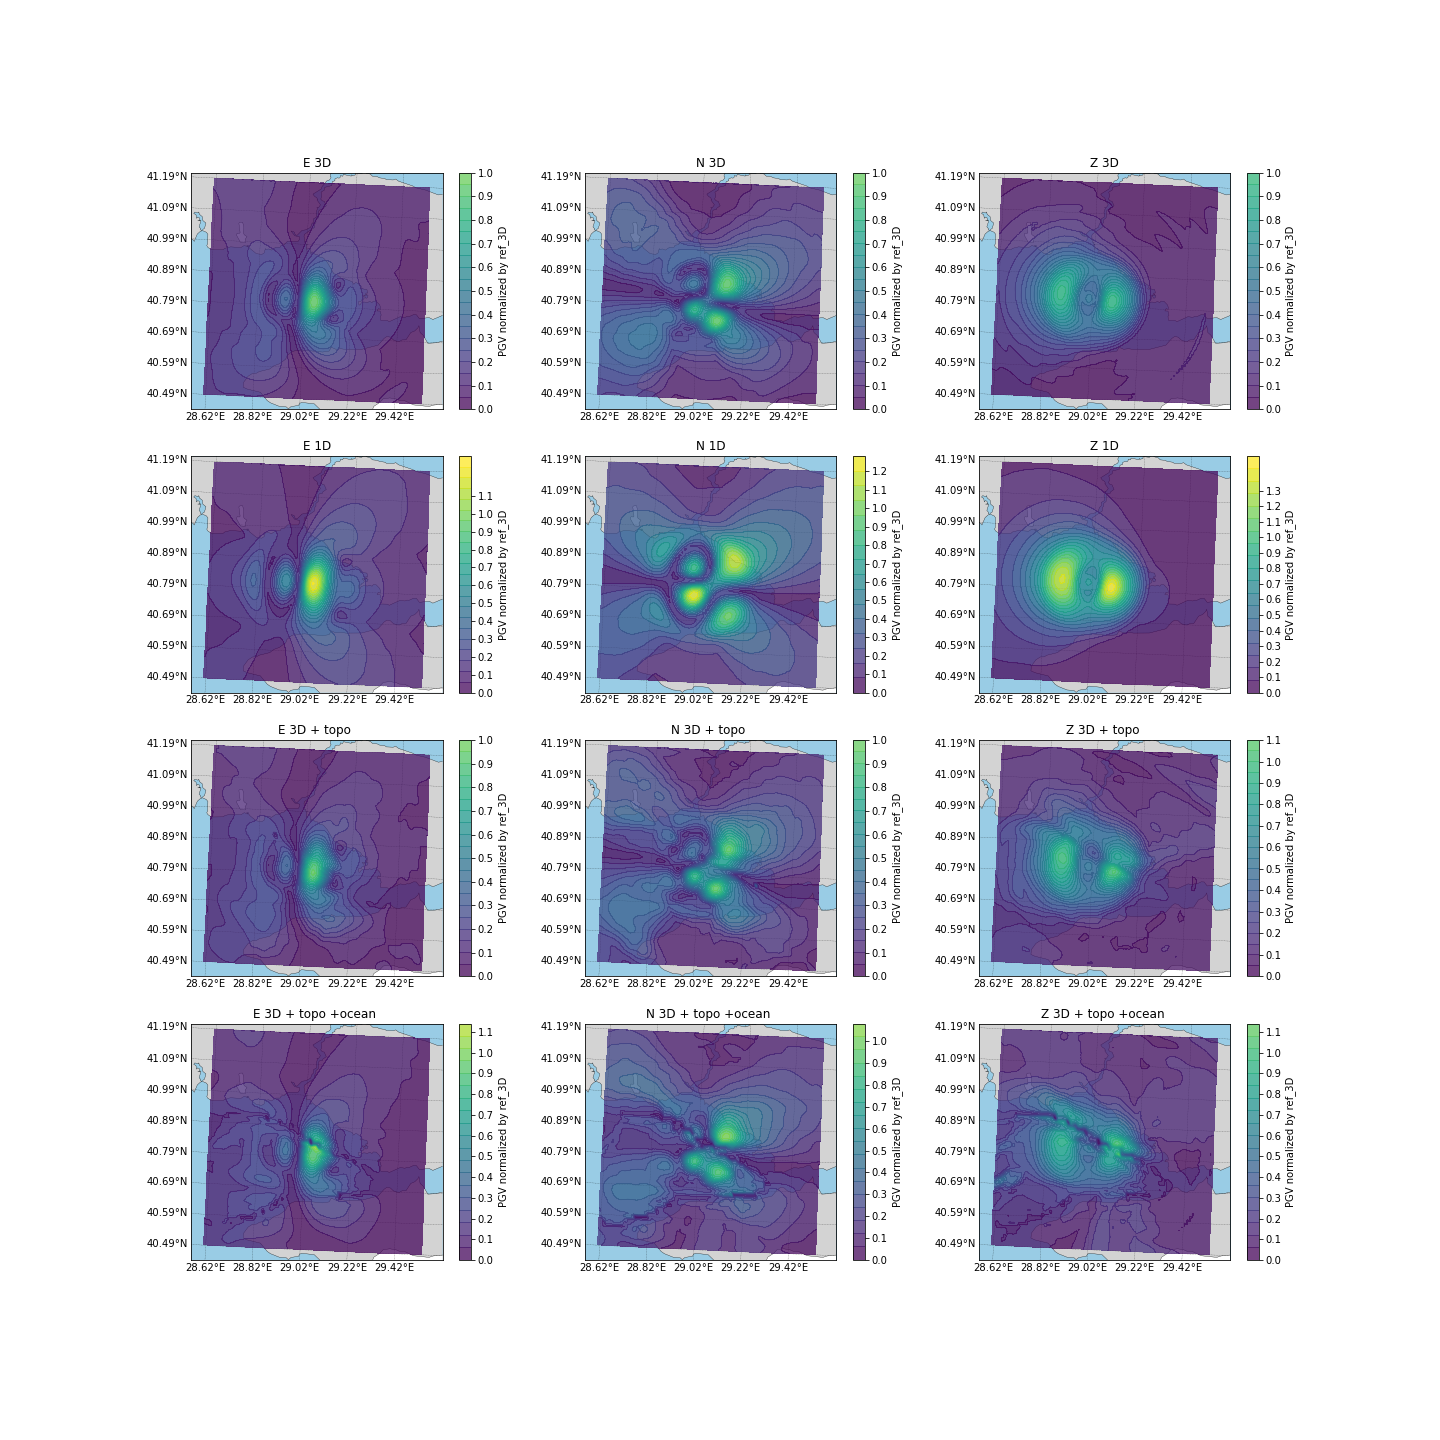
\includegraphics[width=1.2\linewidth]{images_results/Ref_scenarios_normalized_sc3.png}
    \caption{PGV reference scenario CMT3, strike 10, dip 30, rake 90, normalized with respect to the 3D configuration (top row).}
    \label{fig:ref_CMT3}
\end{figure}

\subsubsection{CMT4}

\begin{figure}[h]
    \centering
    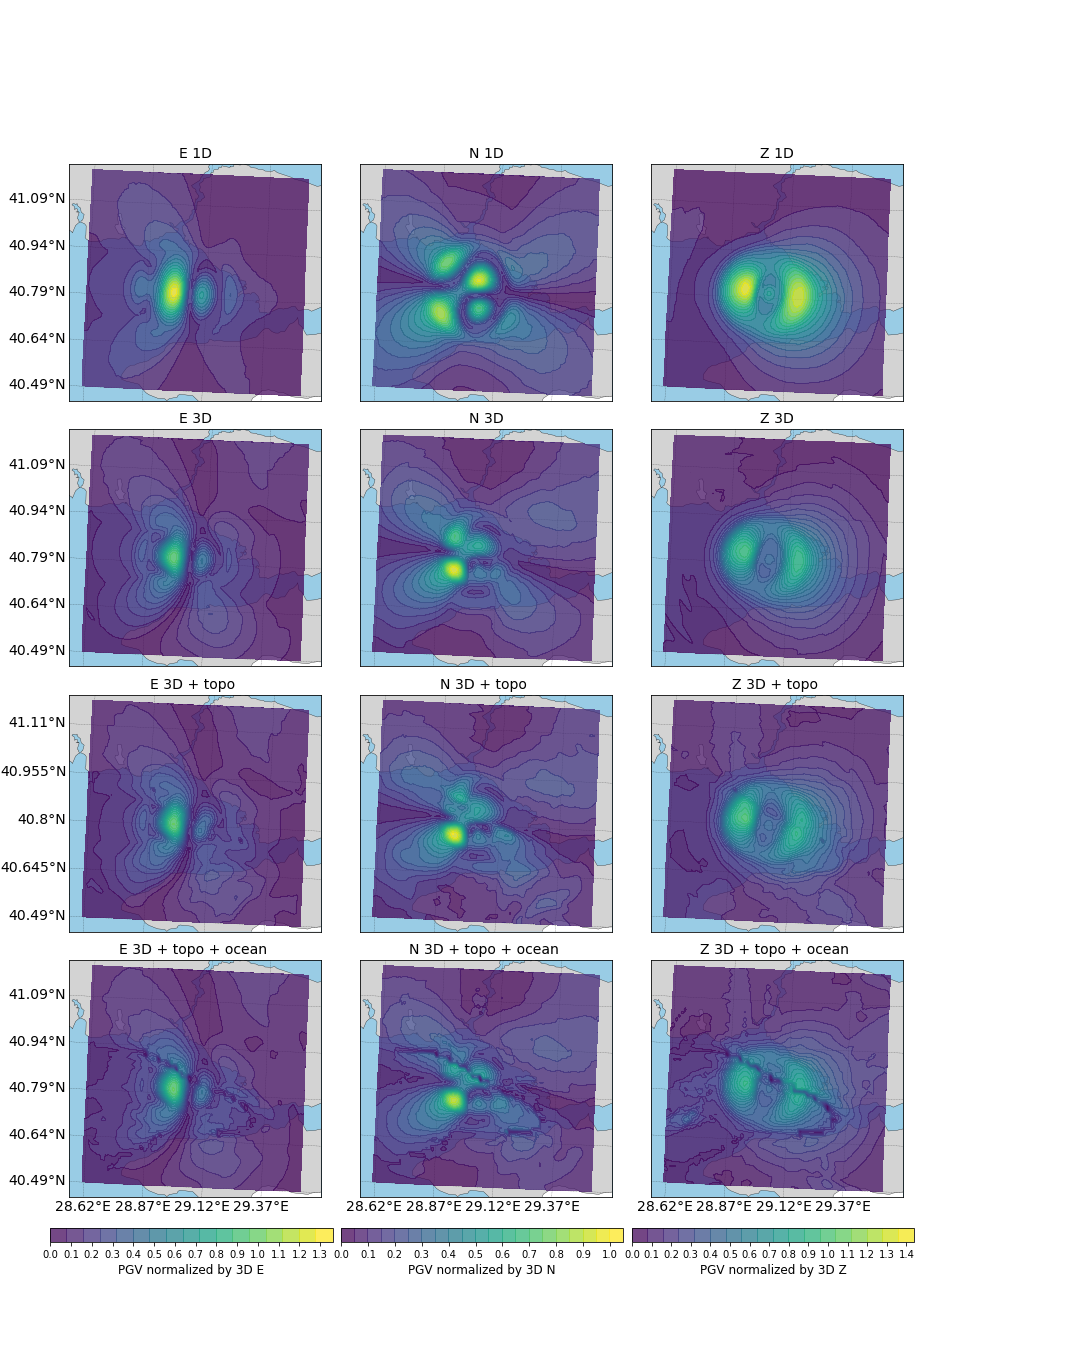
\includegraphics[width=1.2\linewidth]{images_results/Ref_scenarios_normalized_sc4.png}
    \caption{PGV reference scenario CMT4, strike -10, dip 60, rake -90, normalized with respect to the 3D configuration (top row).}
    \label{fig:ref_CMT4}
\end{figure}


\subsection{Variation strike figures CMT3 and CMT4}

\subsubsection{CMT3}
\begin{figure}
    \centering
    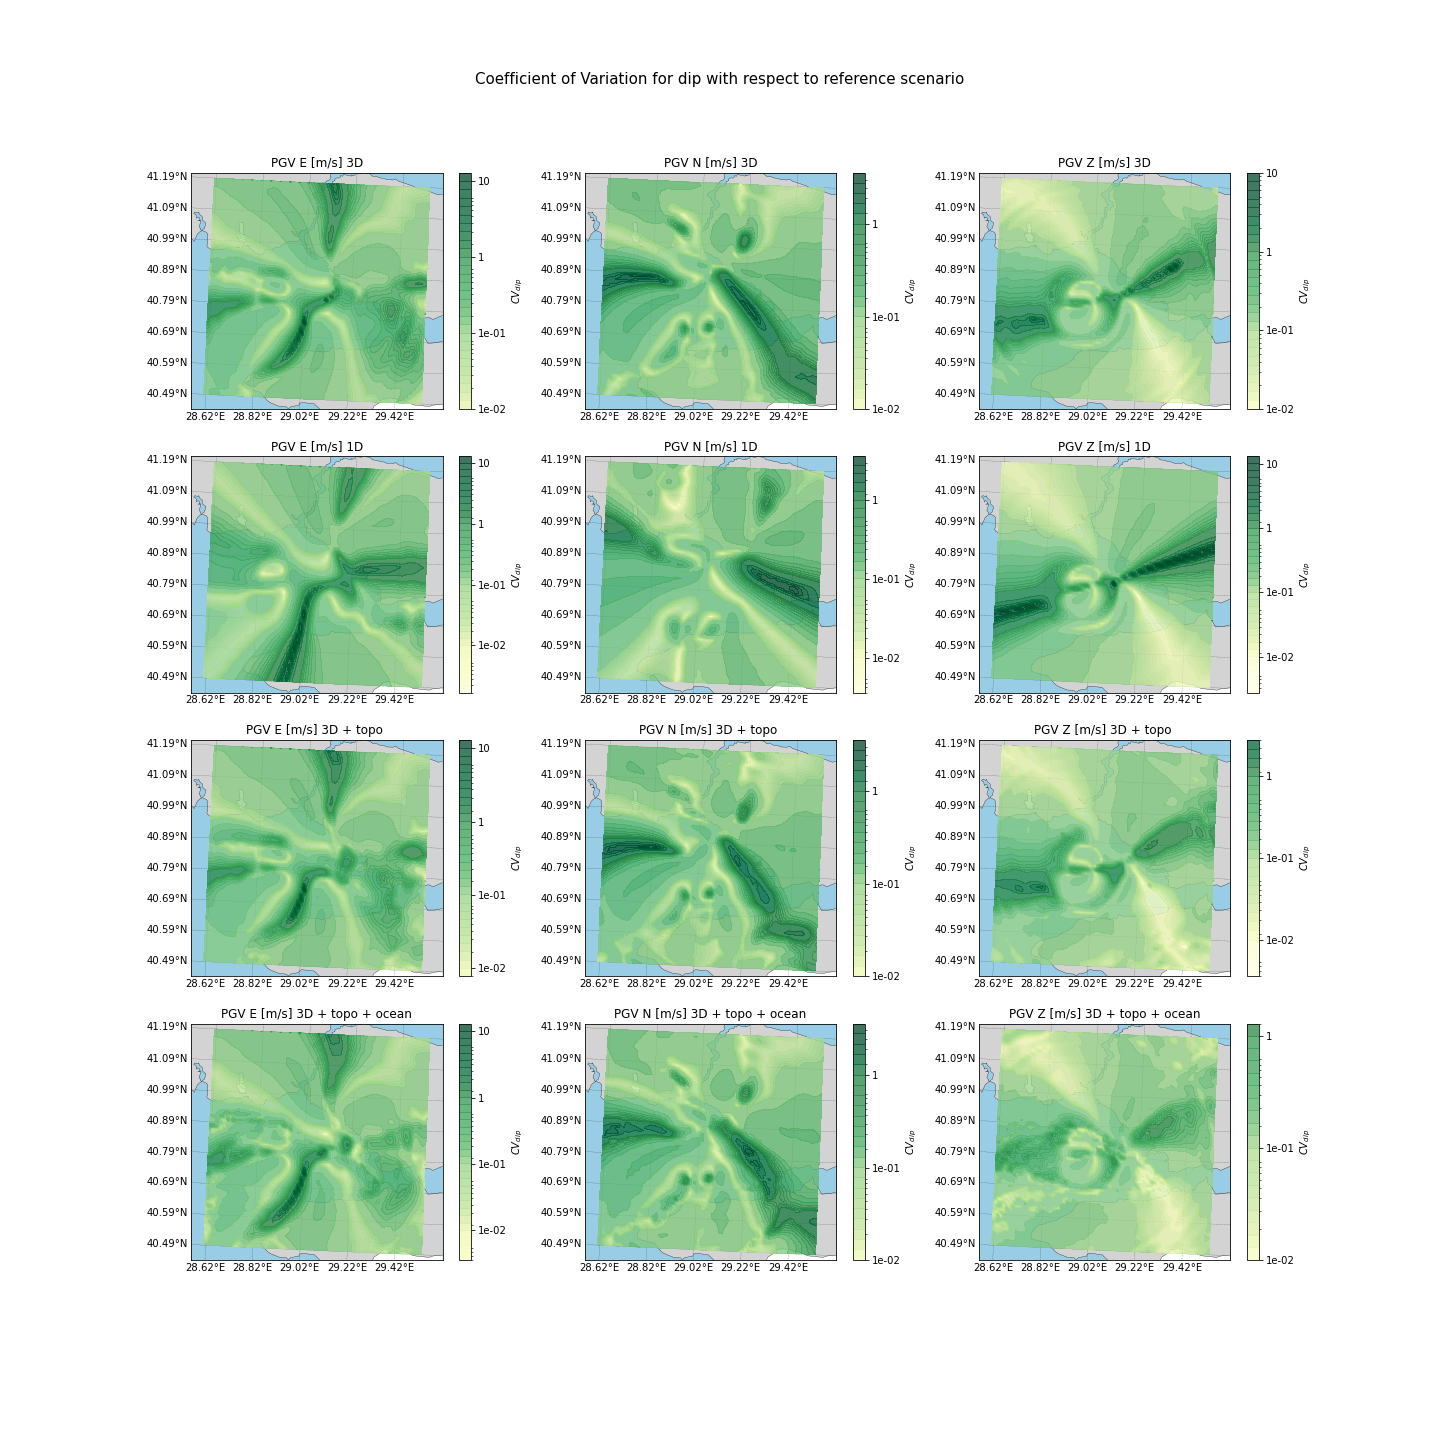
\includegraphics[width=1.2\linewidth]{images_results/dip_variation_sigma_sc2.png}
    \caption{CMT2 coefficient of variation $Cv$ of strike variation, for each model domain in E, N and Z direction. Colourbar set to logarithmic to adequately show the large differences.}
    \label{fig:cmt2sigm}
\end{figure}

\begin{figure}[!h]
    \centering
    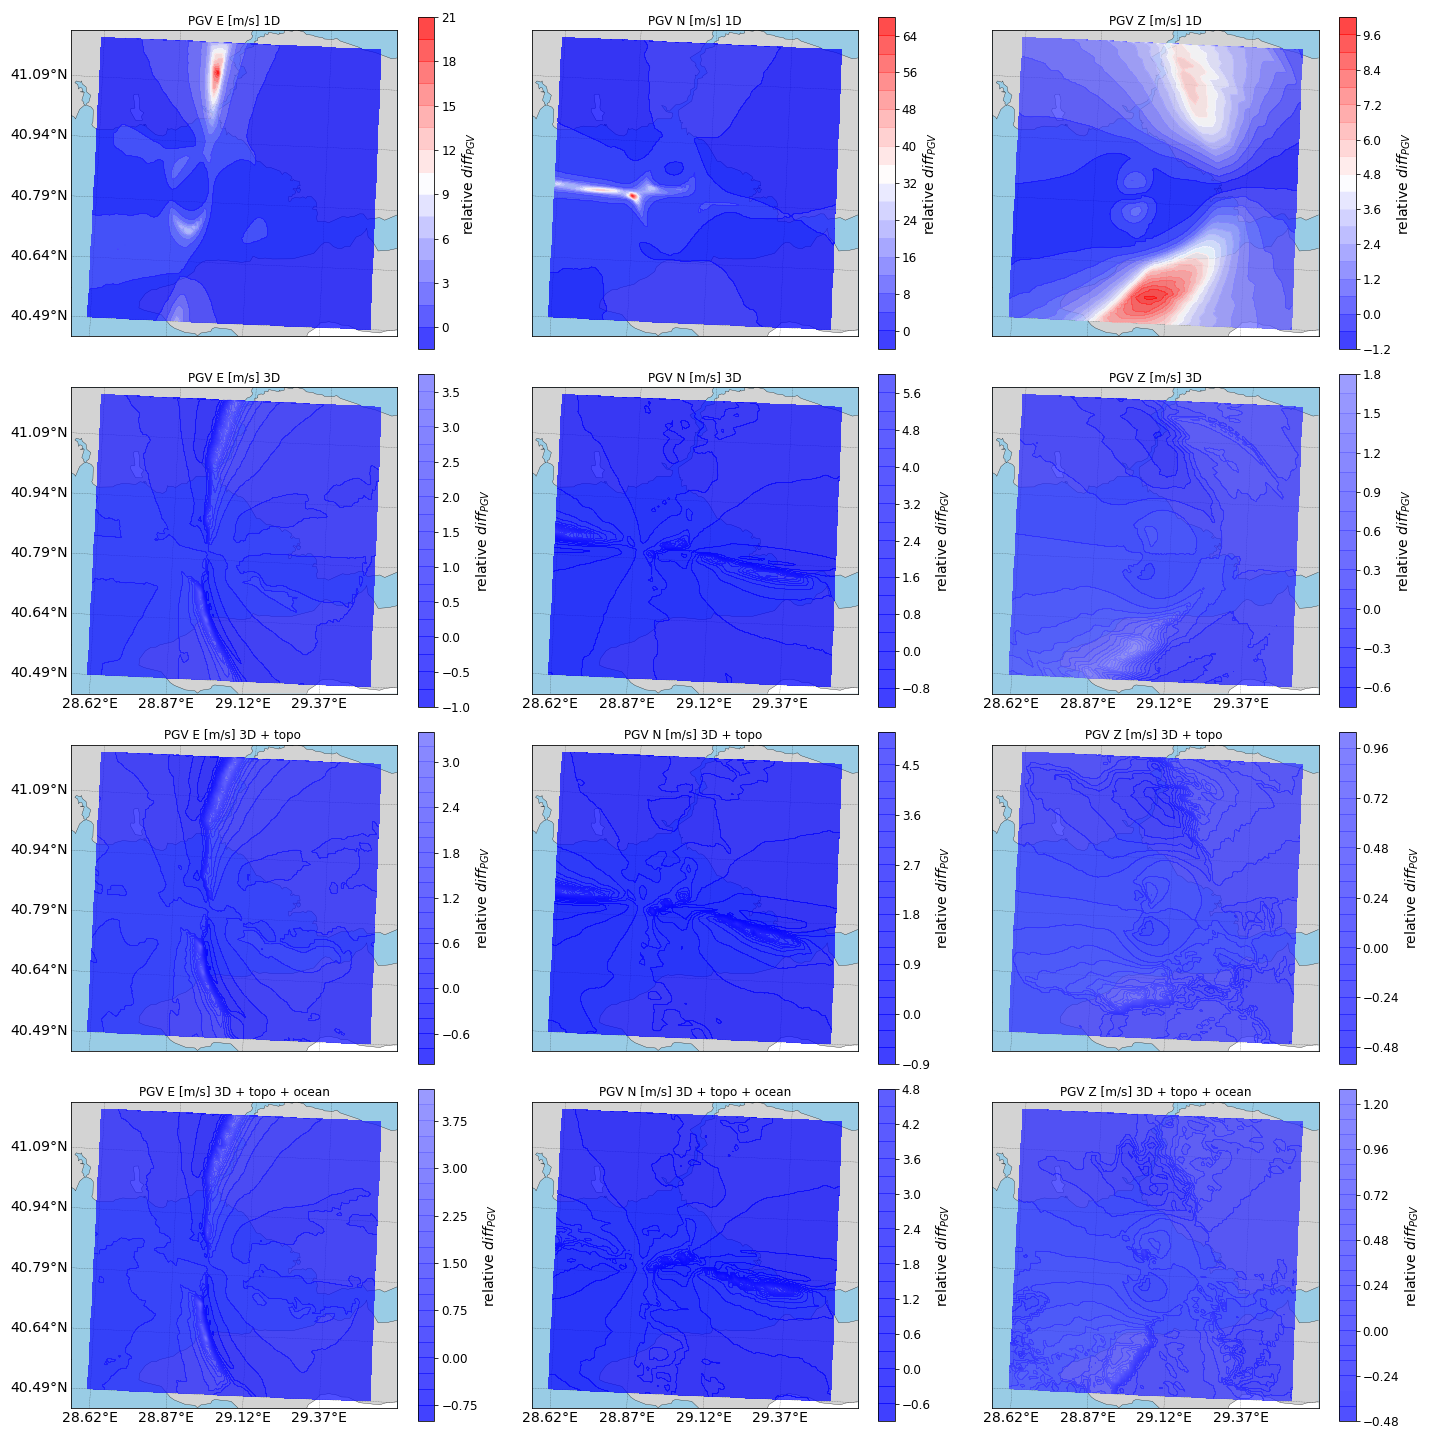
\includegraphics[width=1.2\linewidth]{images_results/strike_variation_epsilon12_sc3.png}
    \caption{CMT3 relative difference between a scenario with a strike variation of 15$\degree$ with respect to the reference scenario. Colorbar set to the total minima and maxima of the 15$\degree$ and 25$\degree$ plots for comparison.}
    \label{fig:ref_eps12-2}
\end{figure}

\begin{figure}[!h]
    \centering
    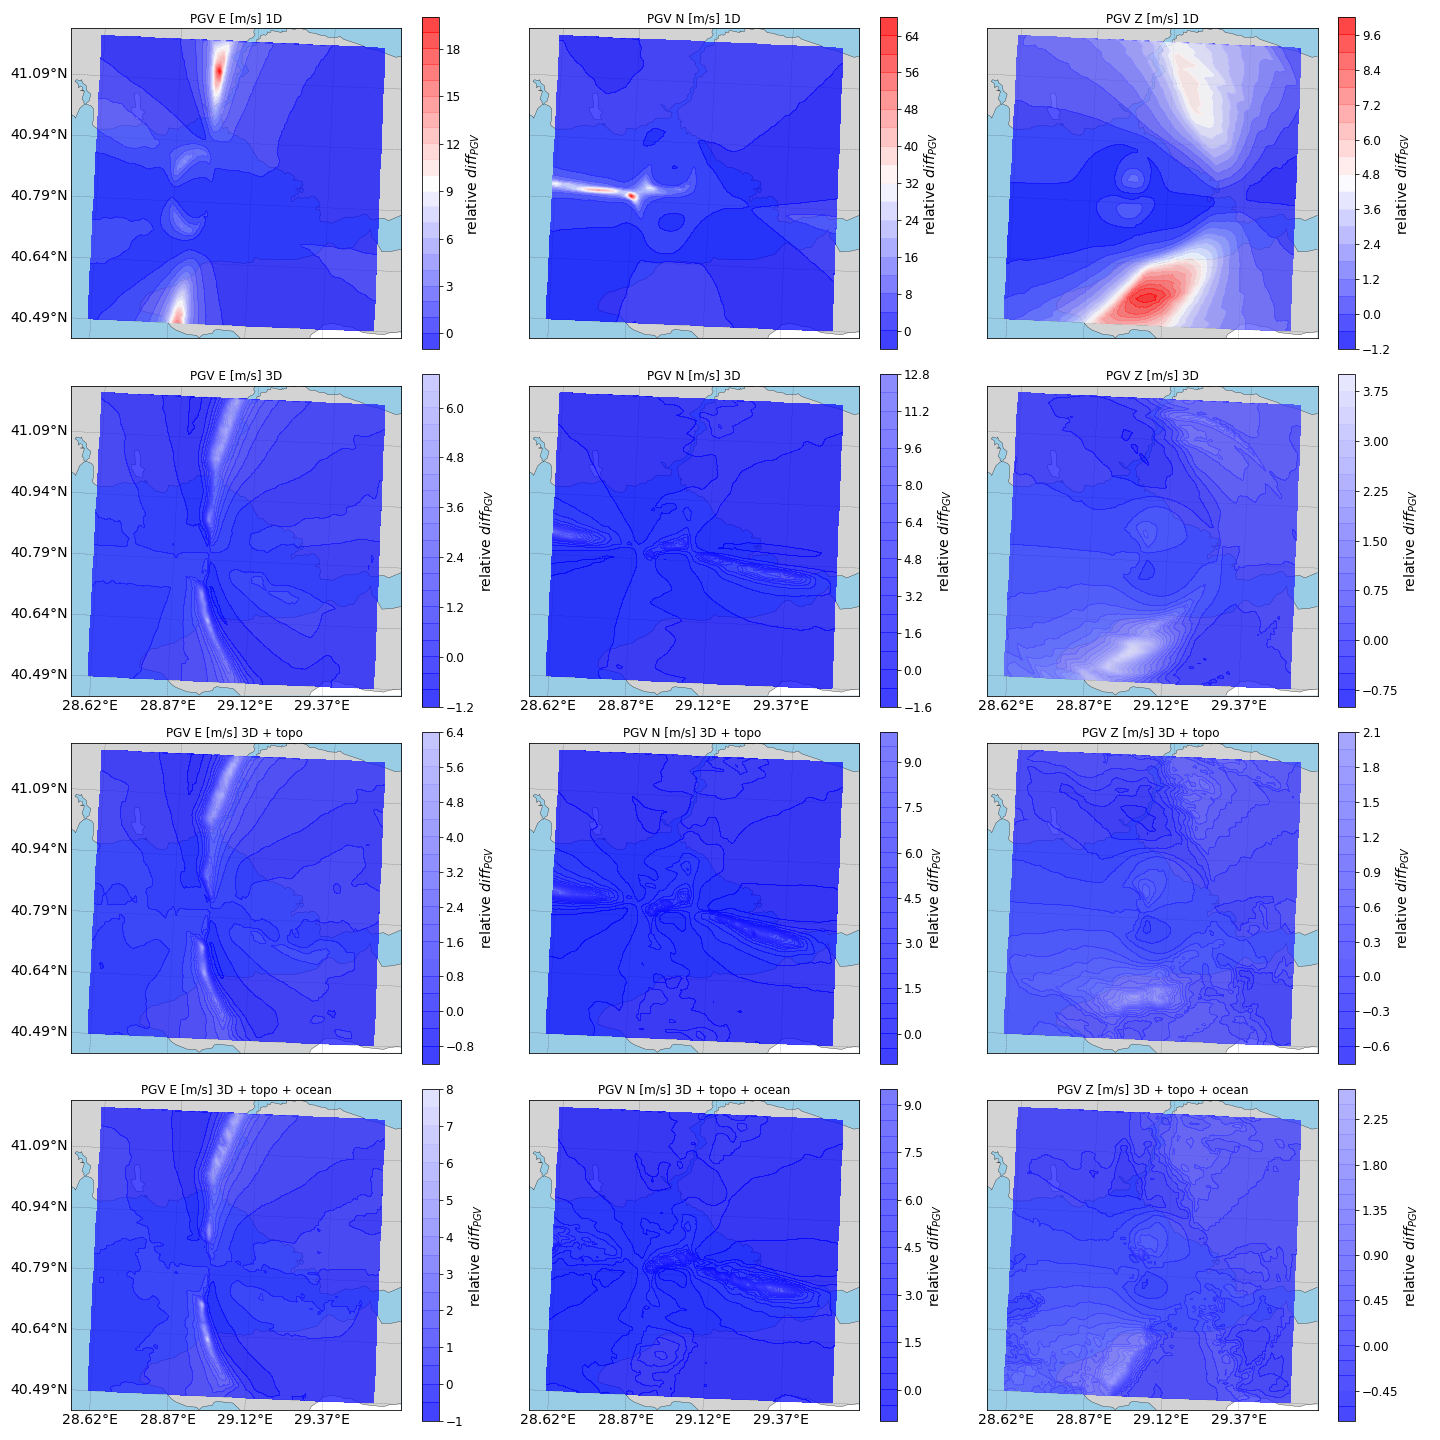
\includegraphics[width=1.2\linewidth]{images_results/strike_variation_epsilon25_sc3.png}
    \caption{CMT3 relative difference between a scenario with a strike variation of 25$\degree$ with respect to the reference scenario. Colorbar set to the total minima and maxima of the 15$\degree$ and 25$\degree$ plots for comparison.}
    \label{fig:ref_eps25-2}
\end{figure}



\subsubsection{CMT4}
\begin{figure}[!h]
    \centering
    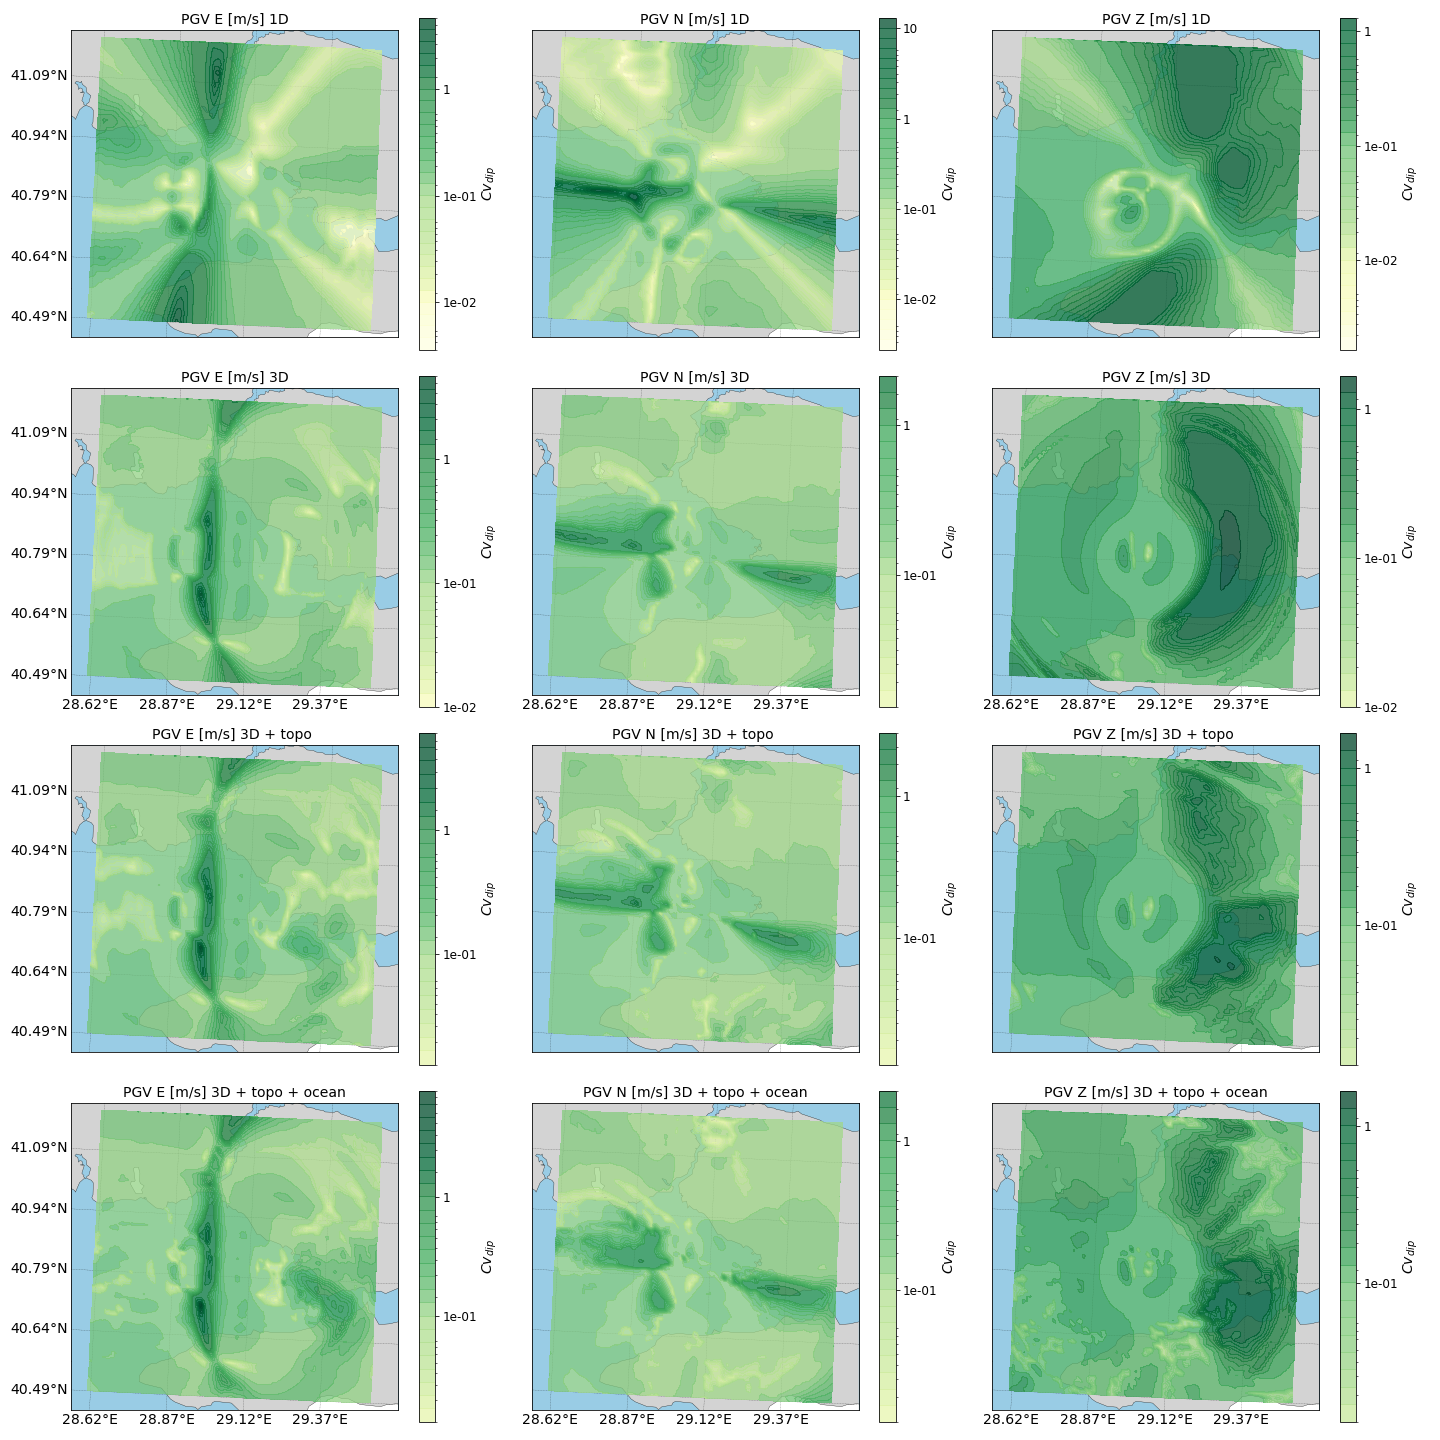
\includegraphics[width=1.2\linewidth]{images_results/dip_variation_sigma_sc3.png}
    \caption{CMT3 coefficient of variation $Cv$ of strike variation, for each model domain in E, N and Z direction. Colourbar set to logarithmic to adequately show the large differences.}
    \label{fig:cmt3sigm}
\end{figure}


\begin{figure}[!h]
    \centering
    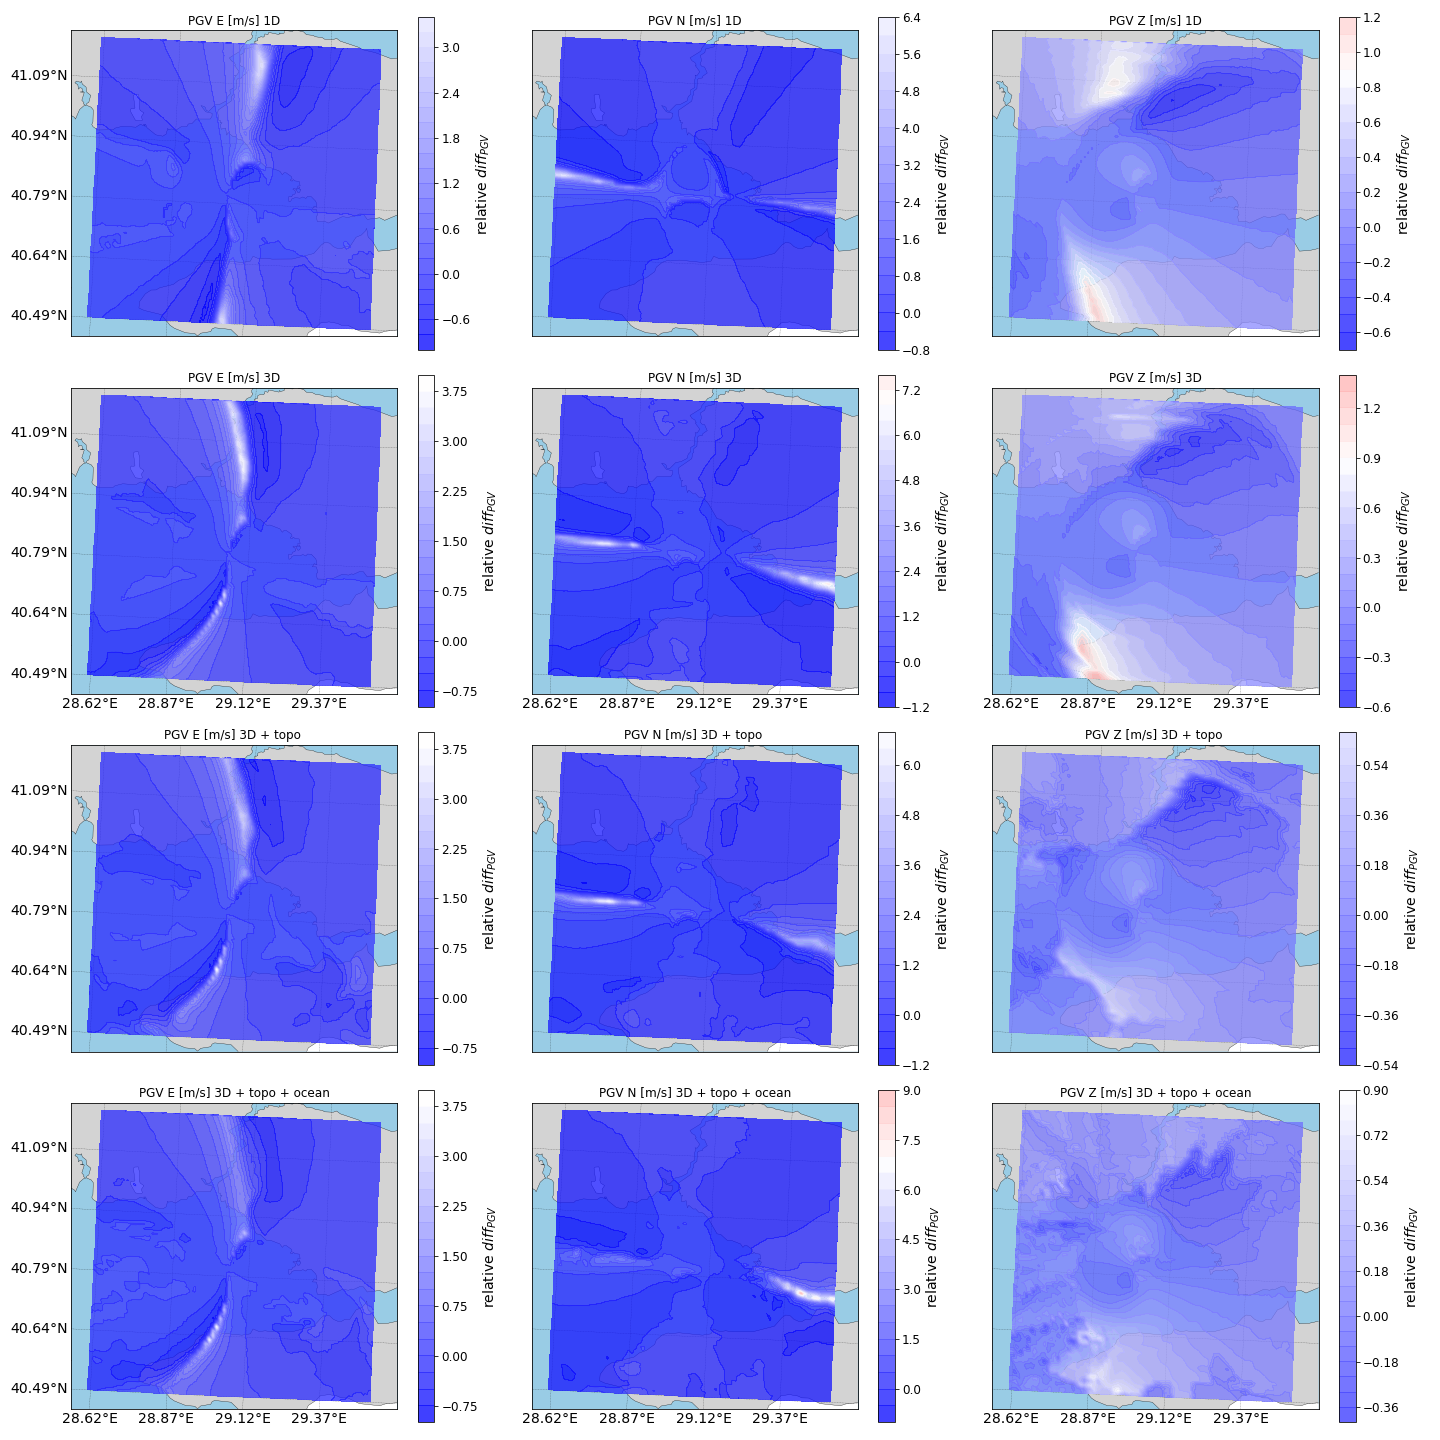
\includegraphics[width=1.2\linewidth]{images_results/strike_variation_epsilon12_sc4.png}
    \caption{CMT4 relative difference between a scenario with a strike variation of 15$\degree$ with respect to the reference scenario. Colorbar set to the total minima and maxima of the 15$\degree$ and 25$\degree$ plots for comparison.}
    \label{fig:ref_eps12-2}
\end{figure}

\begin{figure}[!h]
    \centering
    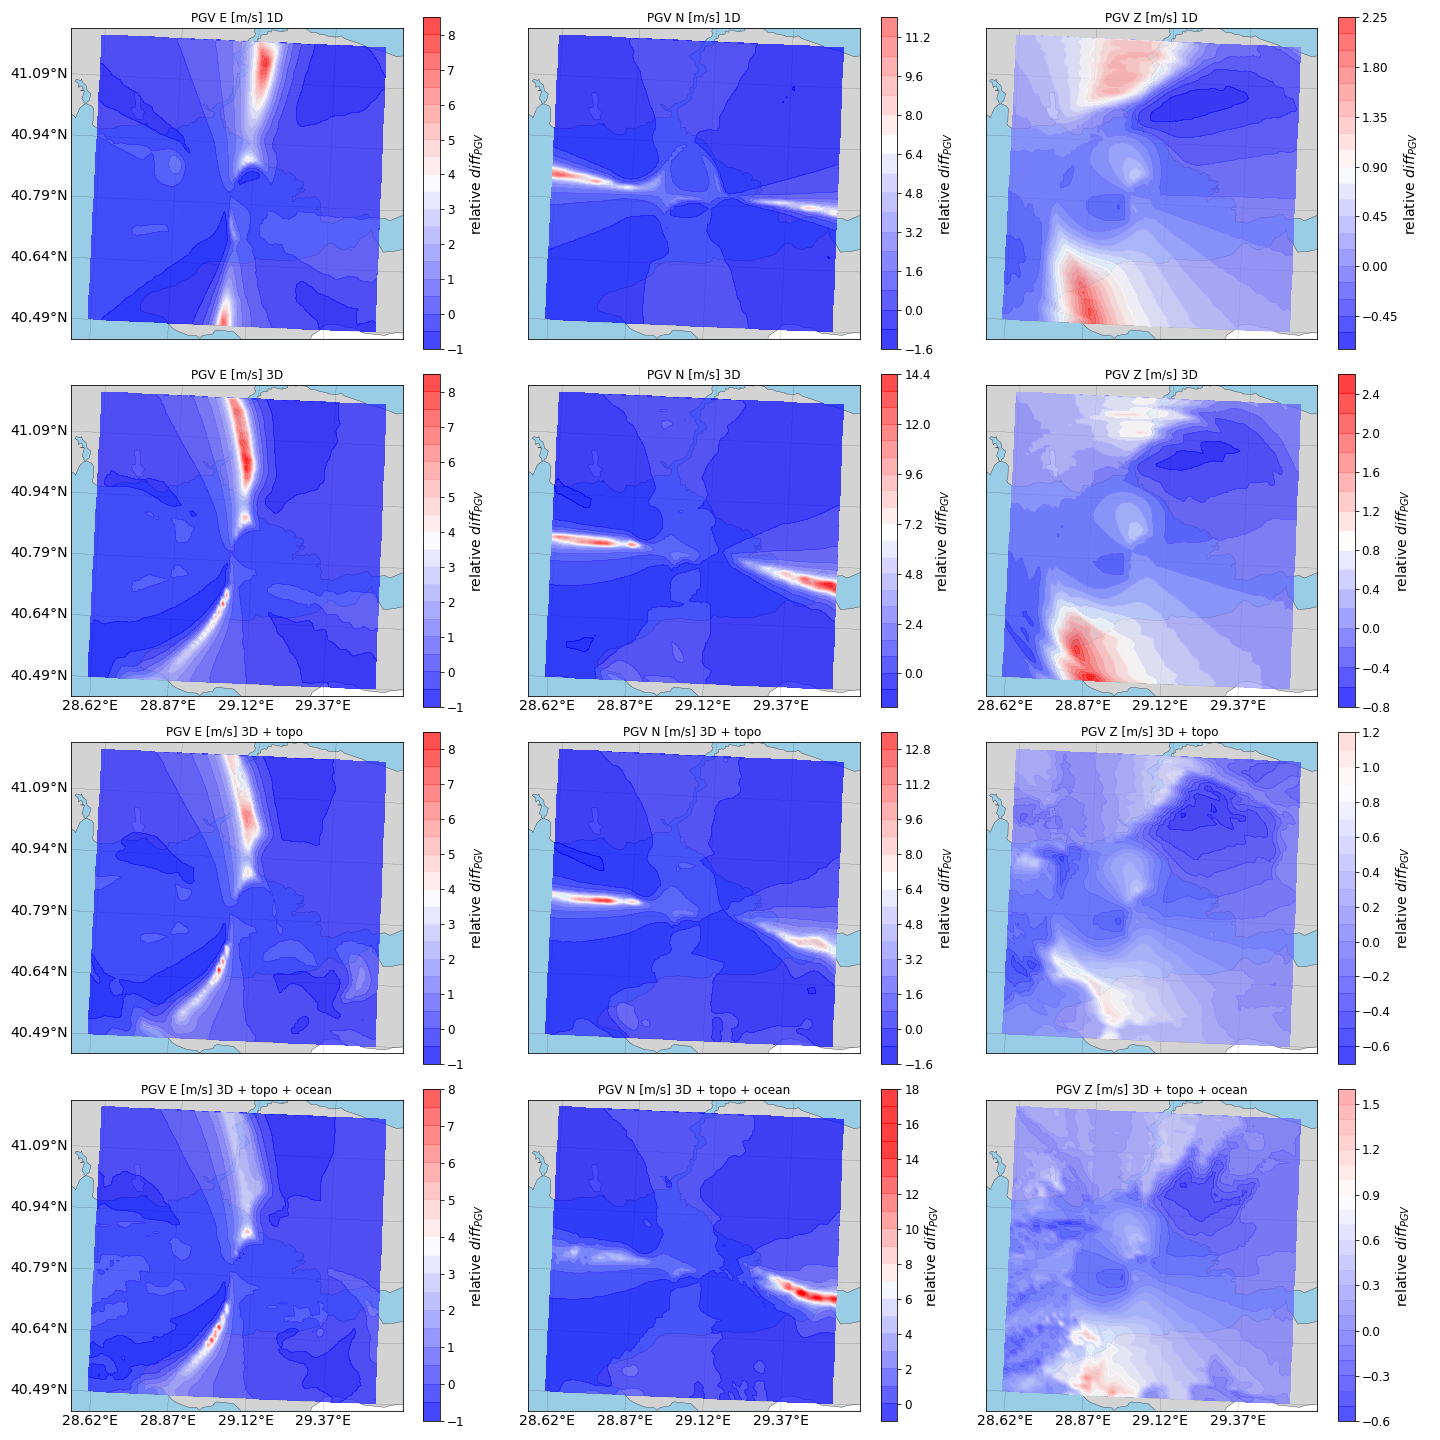
\includegraphics[width=1.2\linewidth]{images_results/strike_variation_epsilon25_sc4.png}
    \caption{CMT4 relative difference between a scenario with a strike variation of 25$\degree$ with respect to the reference scenario. Colorbar set to the total minima and maxima of the 15$\degree$ and 25$\degree$ plots for comparison.}
    \label{fig:ref_eps25-2}
\end{figure}





\section{Other images from results}

\end{document}